\documentclass[a4paper,10pt]{report}
\usepackage[utf8]{inputenc}  
\usepackage[T1]{fontenc}
\usepackage{graphicx}
\usepackage{tikz}
\usepackage[top=2cm, bottom=2cm, left=2cm, right=2cm]{geometry}
\usepackage{hyperref}
\usepackage{multicol}
\usepackage{multirow}
\usepackage{caption}
\usepackage{rotating}
\usepackage{colortbl}

\DeclareUnicodeCharacter{00A0}{ }
\widowpenalty=10000
\clubpenalty=10000


\setlength{\parindent}{0.5cm}
\begin{document}
\begin{multicols}{2}
\title{Etat de lard}
\author{Aurélien Barbotin Pierre David Benjamin Michelland Youna le Vaou}

\maketitle
\chapter{État de l'art}
%opening

\section{Contexte}

Ce projet s'inscrit dans le cadre de notre formation ingénieur. Il s'étend sur six semaines et a été encadré par M. Brodu, chercheur post-doctorant à l'Inria dans l'équipe GeoStat (Géométrie et Statistiques dans les données d'acquisition) à Bordeaux. 

\subsection{Enjeux de la surveillance satellite}

Ce projet se situe dans un domaine particulier de l'utilisation des satellites orbitant autour de la Terre : la classification et le suivi des sols. 
Les applications concernent aussi bien l'agriculture que la surveillance environnementale (fonte des glaces, observation des océans et des forêts) en passant par la géologie, sans oublier la cartographie.

De manière plus concrète, M. Brodu, notre encadrant pédagogique, a mené des projets de traitement d'image satellite pour la surveillance environnementale. Il a notamment travaillé avec l'équipe OptIC (Optimal Inference in Complex and Turbulent Data), associée à l'Inria. L'idée était de suivre l'évolution de la végétation afin de repérer les zones de sécheresse, et ainsi pouvoir mieux gérer les ressources en eau. Une classification des sols de la région autour de Roorkee (Inde) a ainsi été effectuée. 
Cette classification a été réalisée grâce à des données d'imagerie multispectrale, qui est une technique de télédétection. C'est donc à cette technique que nous nous sommes intéressés, même s'il en existe d'autres (imagerie radar par exemple). 

\subsection{Imagerie satellite multispectrale}

Une image photographique couleur "classique" contient en réalité trois images : l'une dans le rouge, l'autre dans le vert et la troisième dans le bleu (RGB en anglais ou RVB en français). Elle ne contient donc que des informations dans le visible. 
\begin{figure}[H]
  \centering
    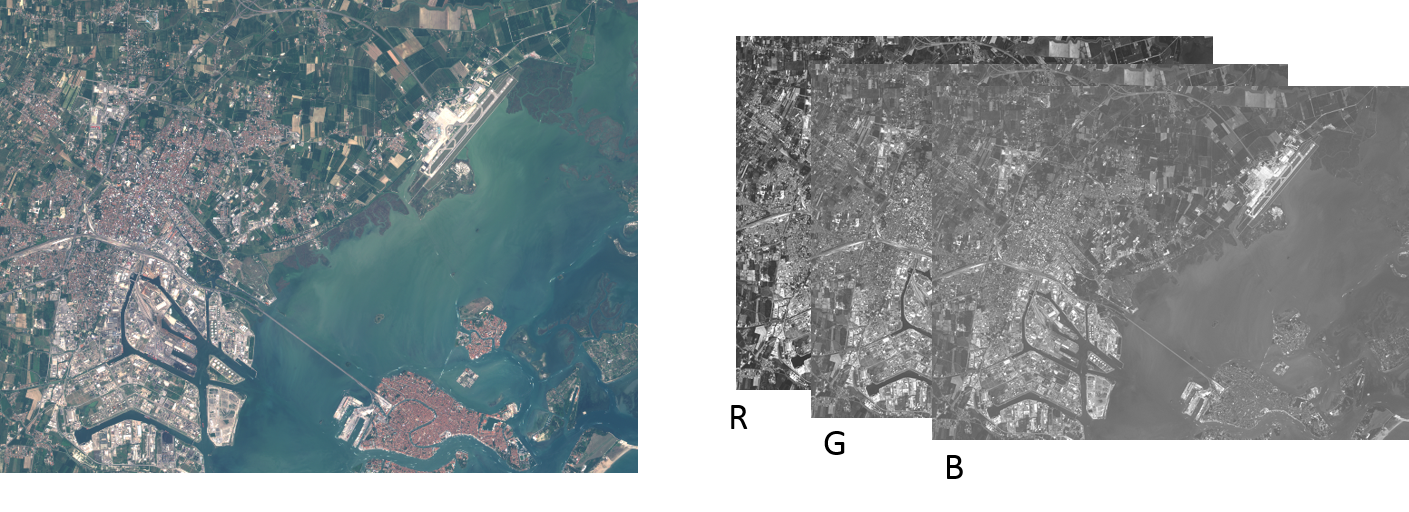
\includegraphics[width=0.75\textwidth]{veniseRGB}
  \caption{Image RGB du Nord de l'Italie (près de Venise)}
  \label{fig:veniseRGB}
\end{figure}

Une image multispectrale, quant à elle, est formée de nombreuses images prises à des longueurs d'ondes variées. Elle contient donc plus d'informations, et selon les longueurs d'ondes d'acquisition peut avoir, en plus du visible, des informations dans l'ultraviolet ou l'infrarouge.

\begin{figure}[H]
  \centering
    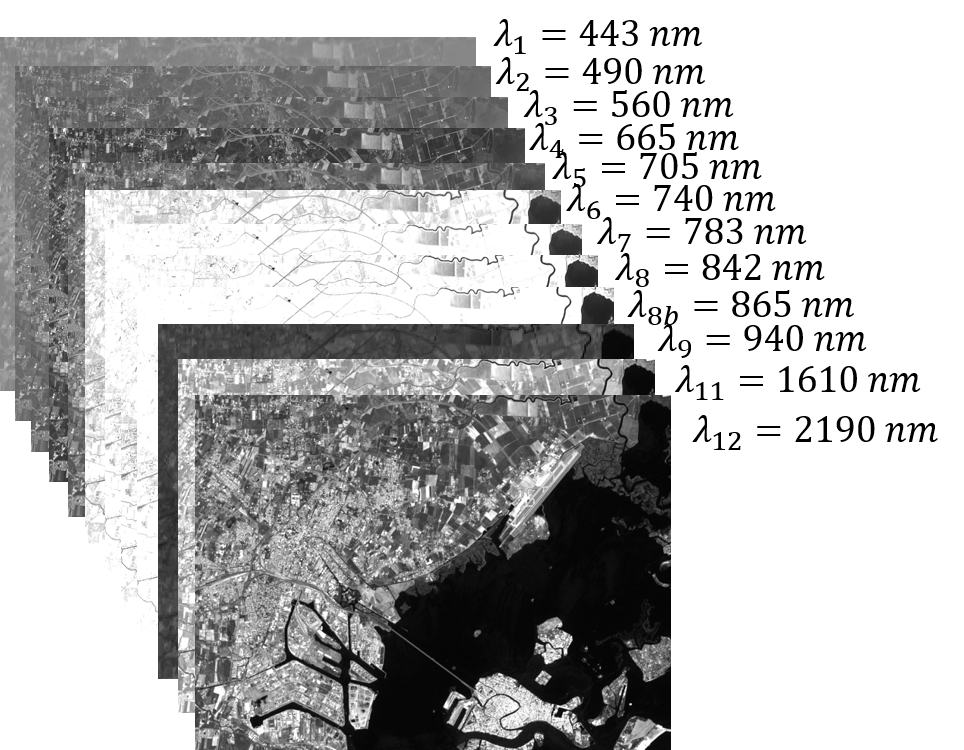
\includegraphics[width=0.5\textwidth]{multispectrale.png}
  \caption{Image multispectrale du Nord de l'Italie (près de Venise)}
  \label{fig:veniseMulti}
\end{figure}

Parmi les satellites utilisant cette technologie on trouve les satellites Aqua et Terra MODIS (Moderate-Resolution Imaging SpectroRadiometer). Ces deux satellites, lancés par la NASA en 1999 et 2002, imagent l'intégralité de la surface de la Terre tous les deux jours. Les données sont ensuite traitées et mises à disposition du public gratuitement, ce qui en a fait une des principales sources d'images satellites multispectrales. Ces satellites sont capables de mesurer 36 bandes fréquentielles avec trois résolutions différentes : 250m, 500m et 1000m par pixel\cite{nasa}. L'objectif de cette mission est de "jouer un rôle vital dans le développement de modèles globaux, validés et interactifs de systèmes terrestres capables de prévoir des changements globaux avec suffisamment de précision pour aider les décideurs politiques à prendre des décisions avisées concernant la protection de notre environnement."

La faible résolution des données MODIS ne permet en revanche pas de discerner des détails comme des cours d'eau ou des habitations, et des données plus précises sont donc nécessaires pour obtenir de meilleures classifications. 

Dans le cadre du projet \textit{Copernicus} d'observation de la Terre, l'agence spatiale européenne (ESA) développe en ce moment les missions Sentinel. Chacune de ces missions consiste en une paire de satellites en orbite autour de notre planète, récoltant des données sur la surface et l'atmosphère. Ainsi, les satellites Sentinel 2 (Sentinel 2-A lancé le 23 juin 2015 et 2-B dont le lancement est prévu pour la seconde moitié de 2016)\cite{sent2} récoltent des données multispectrales sur 13 bandes de fréquence : 4 bandes avec une résolution de 10m/pixel, 6 bandes à 20m/pixel et 3 à 60m/pixel.

\begin{figure}[H]
  \centering
    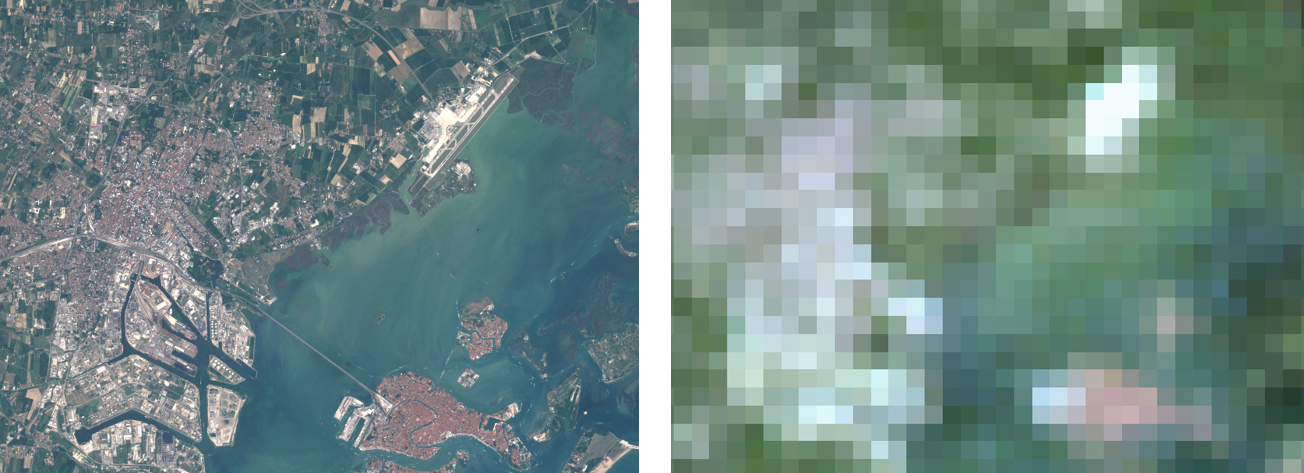
\includegraphics[width=0.75\textwidth]{SentinelVsModis.png}
  \caption{Comparaison d'une image Sentinel 2 (à g.) avec une image MODIS (à d.), en RGB}
  \label{fig:ml}
\end{figure}

Les résolutions de ces images satellites sont donc grandement meilleures que celles acquises par satellites MODIS. Leur mise à disposition du public étant elle aussi gratuite, on comprend leur intérêt. 
Néanmoins, la mission de l'Esa est récente : peu de données sont actuellement disponibles. La courverture temporelle, c'est-à-dire la fréquence à laquelle le satellite passe au-dessus d'une même zone, est également assez faible. Un seul des deux satellites ayant été lancé, le renouvellement des données se fait de manière hebdomadaire, alors que les satellites MODIS renouvellent les données deux fois par jour. 

\subsection{Classification et Machine Learning}

Pour exploiter ces données, il est nécessaire de les classifier. On cherche en effet à distinguer les différentes caractéristiques des sols observés. Les données multispectrales à traiter représentant une quantité très importante, leur classification se fait à travers des algorithmes de "Machine Learning", défini en ces termes : 

\textit{L'apprentissage automatique (Machine Learning en anglais), champ d'étude de l'intelligence artificielle, concerne la conception, l'analyse, le développement et l'implémentation de méthodes permettant à une machine (au sens large) d'évoluer par un processus systématique, et ainsi de remplir des tâches difficiles ou impossibles à remplir par des moyens algorithmiques plus classiques.\footnote{\href{https://fr.wikipedia.org/wiki/Apprentissage_automatique}{Apprentissage automatique}}}

\paragraph{}
Le machine learning se sépare en trois type d'apprentissage :
\begin{itemize}
  \item[>] L'apprentissage non-supervisé, qui consiste à donner à notre algorithme uniquement les données à classifier et à le laisser établir les différentes classes à partir des ensembles qui se séparent le mieux.
  \item[>] La régression, qui cherche à définir les données à l'aide d'une loi mathématique.
  \item[>] L'apprentissage supervisé, pour lequel il faut définir, en plus des données à traiter, des ensembles de vecteurs représentatifs de chacune des classes et déjà classés. Les vecteurs classés manuellement vont servir d’entraînement pour l'apprentissage et donc pour trouver les frontières qui séparent le mieux nos différentes classes.
\end{itemize}

\paragraph{}
Dans le cas de la surveillance d'occupation des sols, on utilise souvent des méthodes supervisées, car il est relativement aisé de reconnaître à l'œil les différents types de zones au sol (eau, champs, villes, ...). Là encore, il existe plusieurs familles d'algorithmes d'apprentissage supervisé, on différenciera dans un premier temps les algorithmes linéaires et non-linéaires. Dans la famille des algorithmes non-linéaire, on trouve des algorithmes intrinsèquement multi-classes (tel que l'algorithme dit des k-plus proches voisins que nous détaillerons plus tard), et les algorithmes binaires.
\label{DiagAlg}
\begin{center}
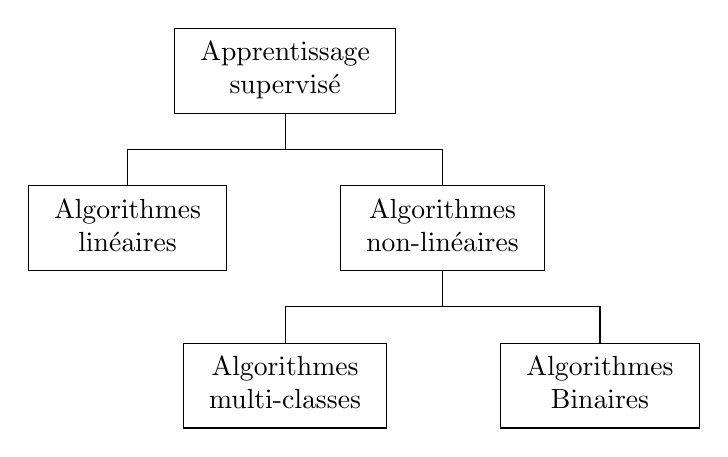
\begin{tikzpicture}
\begin{scope}
\node (AS) at (0,4.9) [rectangle,draw] {\begin{tabular}{c}Apprentissage\\ supervisé\end{tabular} };
\node (ASL) at (-2,2.9) [rectangle,draw] {\begin{tabular}{c}Algorithmes\\ linéaires\end{tabular} };
\node (ASNL) at (2,2.9) [rectangle,draw] {\begin{tabular}{c}Algorithmes\\ non-linéaires\end{tabular} };
\node (ASIM) at (0,0.9) [rectangle,draw] {\begin{tabular}{c}Algorithmes\\ multi-classes\end{tabular} };
\node (ASNM) at (4,0.9) [rectangle,draw] {\begin{tabular}{c}Algorithmes\\Binaires\end{tabular} };
\draw (AS) -- (0,3.9);
\draw (0,3.9) -| (ASNL);
\draw (0,3.9) -| (ASL);
\draw (ASNL) -- (2,1.9);
\draw (2,1.9) -| (ASIM);
\draw (2,1.9) -| (ASNM);
\end{scope}
\end{tikzpicture}
\captionof{figure}{Diagramme des différents algorithme de classification.}
\end{center}
%pas sûr que le diagramme soit utile finalement...
\paragraph{}
Pour les algorithmes intrinsèquement multi-classes, il suffit de stocker les vecteurs d’entraînement et d'appliquer directement la classification à l'ensemble des données, il n'y a donc pas d’entraînement à proprement parler.
\paragraph{}
Les algorithmes binaires, quant à eux, demandent un peu plus de travail. Dès que l'on veut traiter plus de deux classes, il faut faire plusieurs entraînements, en se ramenant chaque fois à un problème binaire. Là encore, il y a deux approches possibles en fonction des algorithmes :
 \begin{itemize}
   \item[>] La première approche s'appelle "un contre tous", elle consiste ,comme son nom l'indique, à prendre chaque classe et à l'opposer à l'ensemble des autres classes. On obtient alors n problèmes binaires et pour un élément à classifier, en cas d'ambiguïté, la classe qui obtient le plus de "votes" favorables est choisie.
   \item[>] La seconde méthode est le "un contre un", toutes les classes sont "opposées" successivement, deux à deux, et de la même façon c'est la classe qui obtient le plus de "votes" favorables qui est choisie. La principale différence réside dans le fait qu'il y ait dans ce cas ${n \choose 2}=\frac{n(n-1)}{2}$ entraînements à réaliser.
 \end{itemize}

\paragraph{L'évaluation\newline}
Pour évaluer la qualité des résultats donnés par ces algorithmes, on procède à une phase d'entraînement suivie d'une phase de test. 
On utilise pour cela un ensemble dont on connaît les classes. On va alors diviser cet ensemble en deux sous-ensembles. Le premier sous-ensemble contiendra à la fois les caractéristiques des points et leurs classes respectives. Il servira à entraîner l'algorithme. Celui-ci va ainsi apprendre quelles sont les caractéristiques de chaque classe. Le deuxième sous-ensemble contiendra uniquement les caractéristiques des points. On pourra ensuite comparer les classes inférées par l'algorithme aux classes attendues. On pourra alors quantifier la qualité des résultats à l'aide de la matrice de confusion correspondante. 

\begin{figure}[H]
  \centering
    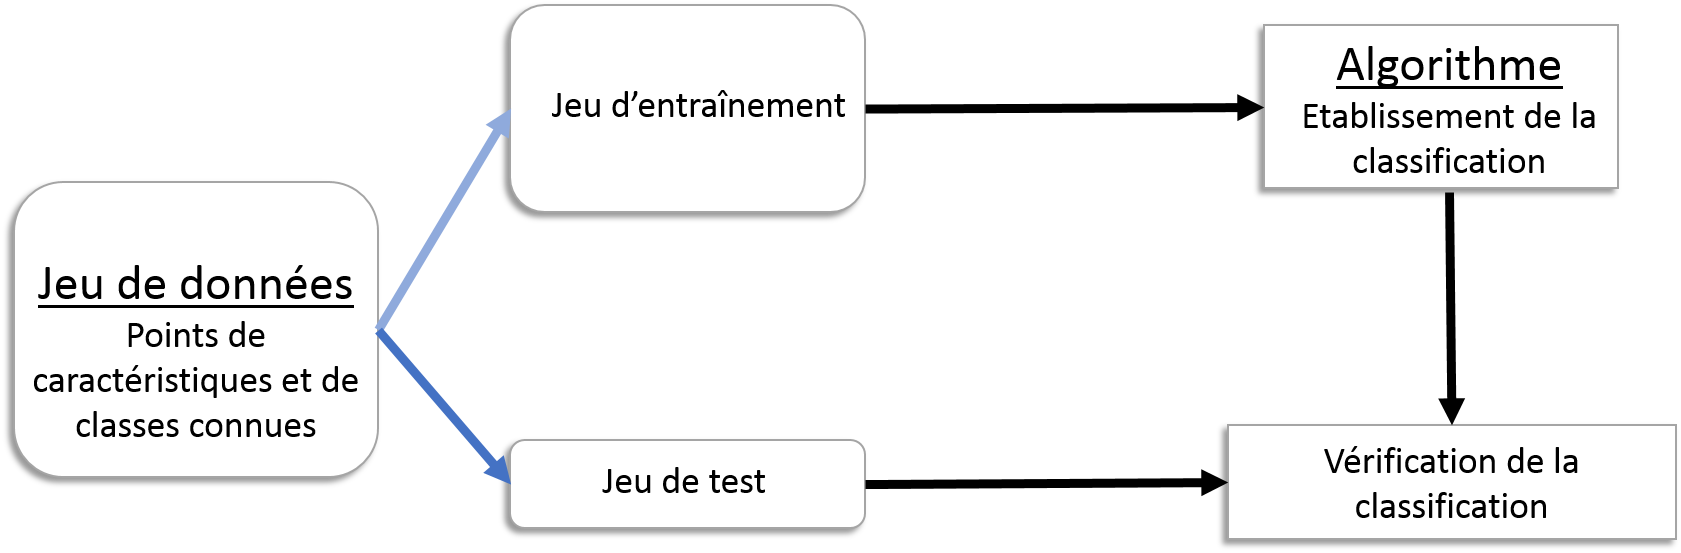
\includegraphics[width=0.75\textwidth]{mlProcess.png}
  \caption{Machine Learning}
  \label{fig:ml}
\end{figure}

\subparagraph{La matrice de confusion\newline}
La matrice de confusion est le principal outil de mesure de la qualité d'une classification. Elle compare en effet la classification prédite par l'algorithme (en lignes) à la classification réelle (en colonnes). \ref{ConfMat}
La diagonale représente le nombre d'éléments bien classés. 
Plusieurs critères sont issus de cette matrice, sous forme de pourcentage. Deux critères sont donnés par classe : la précision (precision) et le rappel (recall). La précision est la quantité d'éléments bien classés, sur le nombre d'éléments réels de cette classe. Le rappel est la quantité d'éléments bien classés, sur le nombre d'éléments prédits par l'algorithme dans cette classe.
Un autre critère est donné de manière global : l'exactitude (accuracy en anglais), qui est la trace de la matrice sur le nombre total d'éléments. Autrement dit, l'exactitude est le pourcentage de données bien classées. C'est principalement ce critère qu'on retiendra.

\begin{figure*}
\caption{Matrice de confusion pour un exemple à trois classes.}
\label{ConfMat}
\begin{center}
\renewcommand{\arraystretch}{3}
\begin{tabular}{|c|c|c|c|c|c|}
\hline
 \multicolumn{2}{|c|}{\multirow{2}{*}{}} & \multicolumn{3}{|c}{Classes Prédites} &  \\
 \cline{3-6}
  \multicolumn{2}{|c|}{} & Classe 1 & Classe 2 & Classe 3 & Précision\\
  \hline
 \multirow{3}{*}{\begin{turn}{90} Classes Théoriques\end{turn}} & Classe 1 & $N_{11}$ & $N_{12}$ & $N_{13}$ & $\frac{N_{11}}{N_{11} + N_{12} + N_{13} }$\\
 \cline{2-6}
  & Classe 2 & $N_{21}$ & $N_{22}$ & $N_{23}$ & $\frac{N_{22}}{N_{21} + N_{22} + N_{23} }$\\
  \cline{2-6}
  & Classe 3 & $N_{31}$ & $N_{32}$ & $N_{33}$ & $\frac{N_{33}}{N_{31} + N_{32} + N_{33} }$\\
  \cline{2-6}
  & Recall  & $\frac{N_{11}}{N_{11} + N_{21} + N_{31} }$ & $\frac{N_{22}}{N_{12} + N_{22} + N_{32} }$ & $\frac{N_{33}}{N_{13} + N_{23} + N_{33} }$ & $\frac{N_{11} + N_{22} + N_{33}}{Nb echantillons}$\footnote {ce résultat donne la fidélité de la classification par rapport à l'image initiale} \\
\hline
\end{tabular}
\end{center}
\end{figure*}



\subsection{Motivation du projet et cahier des charges}

Les données Sentinel 2 étant très récentes, nous faisons partie des premiers à les analyser et aucun article à leur sujet n'a encore été publié. Leur analyse et leur classification relève donc de la recherche. 
Bien que ce projet s'étende sur une durée assez courte (6 semaines), les objectifs fixés étaient :
\begin{itemize}
  \item[>] Définir les principaux intérêts des images multispectrales Sentinel 2.
  \item[>] Etablir une classification de la surface terrestre (suivi d'occupation des sols) en trois classes ("Eau", "Urbain","Champ") à partir d'une image de la base de données Sentinel 2.
  \item[>] Tester les algorithmes de Machine Learning les plus répandus.
\end{itemize}

  Dans un but de répétabilité, nous avons testé et optimisé toutes nos méthodes de machine learning sur une unique image hyperspectrale (dont une vue en RGB est donnée en figure \ref{fig:veniseRGB}).
 

\section{Machine Learning}
\textit{L'apprentissage automatique (machine learning en anglais), champ d'étude de l'intelligence artificielle, concerne la conception, l'analyse, le développement et l'implémentation de méthodes permettant à une machine (au sens large) d'évoluer par un processus systématique, et ainsi de remplir des tâches difficiles ou impossibles à remplir par des moyens algorithmiques plus classiques.\footnote{\href{https://fr.wikipedia.org/wiki/Apprentissage_automatique}{Apprentissage automatique}}}
\subsection{Les principes}
\paragraph{}
Il existe plusieurs familles d'algorithmes qui peuvent être utilisés pour l'apprentissage supervisé, on différenciera dans un premier temps les algorithmes linéaires et non-linéaires. Dans la famille des algorithmes non-linéaire, on trouve des algorithmes intrinsèquement multi-classes (tel que l'algorithme dit des k-plus proches voisins que nous détaillerons plus tard), et les algorithmes binaires.
\label{DiagAlg}
\begin{center}
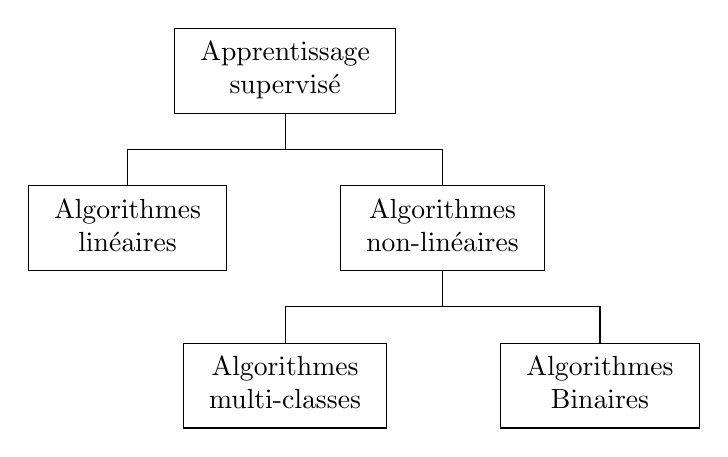
\begin{tikzpicture}
\begin{scope}
\node (AS) at (0,4.9) [rectangle,draw] {\begin{tabular}{c}Apprentissage\\ supervisé\end{tabular} };
\node (ASL) at (-2,2.9) [rectangle,draw] {\begin{tabular}{c}Algorithmes\\ linéaires\end{tabular} };
\node (ASNL) at (2,2.9) [rectangle,draw] {\begin{tabular}{c}Algorithmes\\ non-linéaires\end{tabular} };
\node (ASIM) at (0,0.9) [rectangle,draw] {\begin{tabular}{c}Algorithmes\\ multi-classes\end{tabular} };
\node (ASNM) at (4,0.9) [rectangle,draw] {\begin{tabular}{c}Algorithmes\\Binaires\end{tabular} };
\draw (AS) -- (0,3.9);
\draw (0,3.9) -| (ASNL);
\draw (0,3.9) -| (ASL);
\draw (ASNL) -- (2,1.9);
\draw (2,1.9) -| (ASIM);
\draw (2,1.9) -| (ASNM);
\end{scope}
\end{tikzpicture}
\captionof{figure}{Diagramme des différents algorithme de classification.}
\end{center}

\paragraph{}
Les algorithmes intrinsèquement multi-classes se suffisent à eux même, dans le sens où il suffit d'appliquer l'algorithme à l'ensemble des échantillons d'entraînement pour obtenir une classification complète.
\paragraph{}
Les algorithmes binaires, quand à eux demandent un peu plus de travail, dès que l'on veut traiter plus de deux classe, il faut faire plusieurs entraînements, en se ramenant chaque fois à un problème binaire. La encore, il y deux approches possibles en fonction des algorithmes :
 \begin{itemize}
   \item[>] La première approche est appelé un contre tous, elle consiste comme son nom l'indique, à prendre chaque classe et à l'opposer à l'ensemble des autres classes. On obtient alors n problèmes binaires et pour un élément à classifier, en cas d'ambiguïté, la classe qui obtient le plus de "votes" favorables est choisie;
   \item[>] La seconde méthode est celle du un contre un, toutes les classes sont "opposées" successivement, deux à deux, et de la même façon c'est la classe qui obtient le plus de "votes" favorables qui est choisie. La principale différence réside dans le fait qu'il y a dans ce cas ${n \choose 2}=\frac{n(n-1)}{2}$ entraînements à réaliser.
 \end{itemize}
 \subsection{Les algorithmes}
\paragraph{Les classifications linéaires\\}
Réaliser une classification linéaire d'un ensemble de données en différentes classes revient, en deux dimensions, à trouver la droite qui sépare au mieux deux ensembles de vecteurs.
\label{ClassLin}
\begin{center}
 \begin{tikzpicture}
 \begin{scope}
 \draw[latex-latex, thin, draw=gray] (-4,0)--(4,0) node [right] {$x$}; % l'axe des abscisses
 \draw[latex-latex, thin, draw=gray] (0,-4)--(0,4) node [above] {$y$}; % l'axe des ordonnées
 \draw[thick] (-4,-4)--(4,4); % la courbe

\foreach \Point in {(-2,2), (-2,1.8), (-2,2.2), (-1.5,2), (-1.8,2.2),(-1.5,2.2),(-1.8,2),(-2.2,2),(-2,1.5),(-1.8,1.8)}{
    \node [blue] at \Point {\textbullet};
}

\foreach \Point in {(2,-2), (2,-1.8), (2,-2.2), (1.5,-2), (1.8,-2.2),(1.5,-2.2),(1.8,-2),(2.2,-2),(2,-1.5),(1.8,-1.8)}{
    \node [red] at \Point {\textbullet};
}

% to ensure that the points are being properly centered:
\draw [dotted, gray] (-4,-4) grid (4,4);
 \end{scope}
\end{tikzpicture}
\captionof{figure}{Illustration du principe de la classification linéaire.}
\end{center}

il existe plusieurs méthodes pour trouver une droite qui sépare correctement les deux ensembles de points :
\begin{itemize}
  \item[>] La première méthode consiste à faire l'hypothèse que tous les points des deux ensembles sont alignés, et qu'on peut alors trouver une droite telle que tous les points soient à une distance de 1, pour l'une des deux classes, et de -1 pour l'autre. On se ramène alors à une optimisation linéaire qui peut-être résolue par la méthode des moindres carrés.
  \item[>] Une seconde méthode consiste à utiliser l'analyse discriminante linéaire\footnote{ou analyse discriminante de Fisher}(LDA), c'est-à-dire poser l'hypothèse que chaque ensemble de points à une distribution gaussienne, et à trouver, à partir de la variance et de la moyenne de ces distributions la meilleure séparation entre les ensembles. Cependant, cette hypothèse nous pousse à considérer uniquement un apprentissage de type un contre un et donc à faire plus d'entraînement.
\end{itemize}
\paragraph{Les classification non-linéaires}
\subparagraph{Machine à Vecteurs de Support (SVM) :}

Les SVM ont été développées dans les années 1990 d'après les travaux de Vladimir Vapnik, elle généralise les classificateurs linéaires en cherchant une séparation linéaire de marge maximum, mais en augmentant la dimension de l'espace d'étude. Par l'astuce du \textit{kernel trick}\cite{aizermanSVM}, qui consiste à remplacer le produit scalaire de l'espace considéré par l'évaluation d'une fonction, on peut ramener l'étude d'un problème non séparable linéairement, à un problème linéaire. Une classification basée sur les SVM admet donc des méta-paramètres, qui devront être fixés par l'utilisateur avant de réaliser l'entraînement. Pour optimiser au mieux ses paramètres, on utilise une méthode d'évaluation dite validation croisée qui est expliqué plus en détails par la suite\footnote{voir le paragraphe : L'évaluation}
\subparagraph{Les K plus proches voisins :}
\subsection{L'évaluation}
\paragraph{La matrice de confusion\newline}
La matrice de confusion est le principal outil de mesure de la qualité d'une classification. Pour la construire, il faut, dans un premier temps fournir un ensemble de données, dont on connaît déjà la classe, et dont on va classifier les éléments. La matrice de confusion va alors servir à synthétiser toutes les informations que l'on peut en tirer.\ref{ConfMat}
\begin{figure*}
\caption{Matrice de confusion pour un exemple à trois classes.}
\label{ConfMat}
\begin{center}
\renewcommand{\arraystretch}{3}
\begin{tabular}{|c|c|c|c|c|c|}
\hline
 \multicolumn{2}{|c|}{\multirow{2}{*}{}} & \multicolumn{3}{|c}{Classes Prédites} &  \\
 \cline{3-6}
  \multicolumn{2}{|c|}{} & Classe 1 & Classe 2 & Classe 3 & Précision\\
  \hline
 \multirow{3}{*}{\begin{turn}{90} Classes Théoriques\end{turn}} & Classe 1 & $N_{11}$ & $N_{12}$ & $N_{13}$ & $\frac{N_{11}}{N_{11} + N_{12} + N_{13} }$\\
 \cline{2-6}
  & Classe 2 & $N_{21}$ & $N_{22}$ & $N_{23}$ & $\frac{N_{22}}{N_{21} + N_{22} + N_{23} }$\\
  \cline{2-6}
  & Classe 3 & $N_{31}$ & $N_{32}$ & $N_{33}$ & $\frac{N_{33}}{N_{31} + N_{32} + N_{33} }$\\
  \cline{2-6}
  & Recall  & $\frac{N_{11}}{N_{11} + N_{21} + N_{31} }$ & $\frac{N_{22}}{N_{12} + N_{22} + N_{32} }$ & $\frac{N_{33}}{N_{13} + N_{23} + N_{33} }$ & $\frac{N_{11} + N_{22} + N_{33}}{Nb echantillons}$\footnote {ce résultat donne la fidélité de la classification par rapport à l'image initiale} \\
\hline
\end{tabular}
\end{center}
\end{figure*}

\newpage
\paragraph{La validation croisée\newline}
Il s'agit d'une technique d'évaluation de la classification qui va nous permettre de maximiser la taille des polygones d'entraînement et de test. En effet, cette technique consiste à n'avoir qu'un seul jeu de polygones qui seront utilisés intégralement pour le test et pour l'entraînement. L'astuce réside ici à utiliser une partie des éléments du polygone pour l'entraînement et le reste pour le test, puis de réitérer en changeant les éléments utilisés pour le test et ainsi de suite jusqu'à ce que tous les éléments aient été utilisé pour le test.
\begin{center}
\renewcommand{\arraystretch}{4}
\begin{tabular}{c | c || c || c}
  Etape 1& Etape 2 & Etape 3\\
  \cellcolor{Periwinkle}test & \cellcolor{NavyBlue}entrainement & \cellcolor{NavyBlue}entrainement\\
  \cellcolor{NavyBlue}entrainement & \cellcolor{Periwinkle}test & \cellcolor{NavyBlue}entrainement\\
  \cellcolor{NavyBlue}entrainement & \cellcolor{NavyBlue}entrainement & \cellcolor{Periwinkle}test\\
\end{tabular}
  \captionof{figure}{Illustration de la validation croisée.}
\end{center}

\subsection{Les logiciels de classification}
\paragraph{QGIS}
\paragraph{}
QGIS est un logiciel libre multiplateforme, qui permet de traiter les formats usuels d'image satellite, mais aussi d'y ajouter des couches vectorielles pour délimiter des polygones ou classifier des zones géographiques.
De plus, la communauté de QGIS a développé de nombreux plugins permettant d'appliquer différents algorithmes de machine learning.\newline
Le logiciel SAGA, intégré à QGIS, utilise l'algorithme de ressemblance maximale, qui permet de faire une classification statistique des pixels, ayant choisi des polygones d’entraînement, ils vont être assimilés à des lois normales et à partir de leurs moyennes et de leurs variances, les pixel inconnus vont appartenir à la classe à laquelle ils ont le plus de chance d'appartenir.
Semi-Automatic Classification Plugin, permet également d'obtenir des classifications à partir d'image à l'aide de différents algorithmes.
OrfeoToolBox est un autre logiciel qui a la possibilité d'être utilisé via Qgis et qui peut réaliser une classification d'images satellite.

\paragraph{ENVI}\footnote{\href{http://www.exelisvis.fr/ProduitsetServices/LesproduitsENVI/ENVI.aspx}{ENVI}}
\paragraph{}
ENVI est un logiciel propriétaire payant sous licence commerciale. Il permet de traiter efficacement les données satellite à l'aide de plusieurs algorithmes dont celui de la ressemblance maximum.
\paragraph{}

\chapter{Implémentation}
\section{C++ :}
\paragraph{Les moindres carrés}
Le premier algorithme à être implémenté en C++ a été celui des moindres carrés, en effet, il est relativement simple à coder si l'on utilise une bibliothèque vectorielle comme eigen qui inclue différentes méthodes de résolution des problèmes linéaires. Nous avons ainsi pu observer notre première image de classification.\ref{firstLSE}\ref{veniseLSE}
\begin{figure*}
\begin{center}
  \caption{Première classification obtenue à l'aide des moindres carrés.}
  \label{firstLSE}
  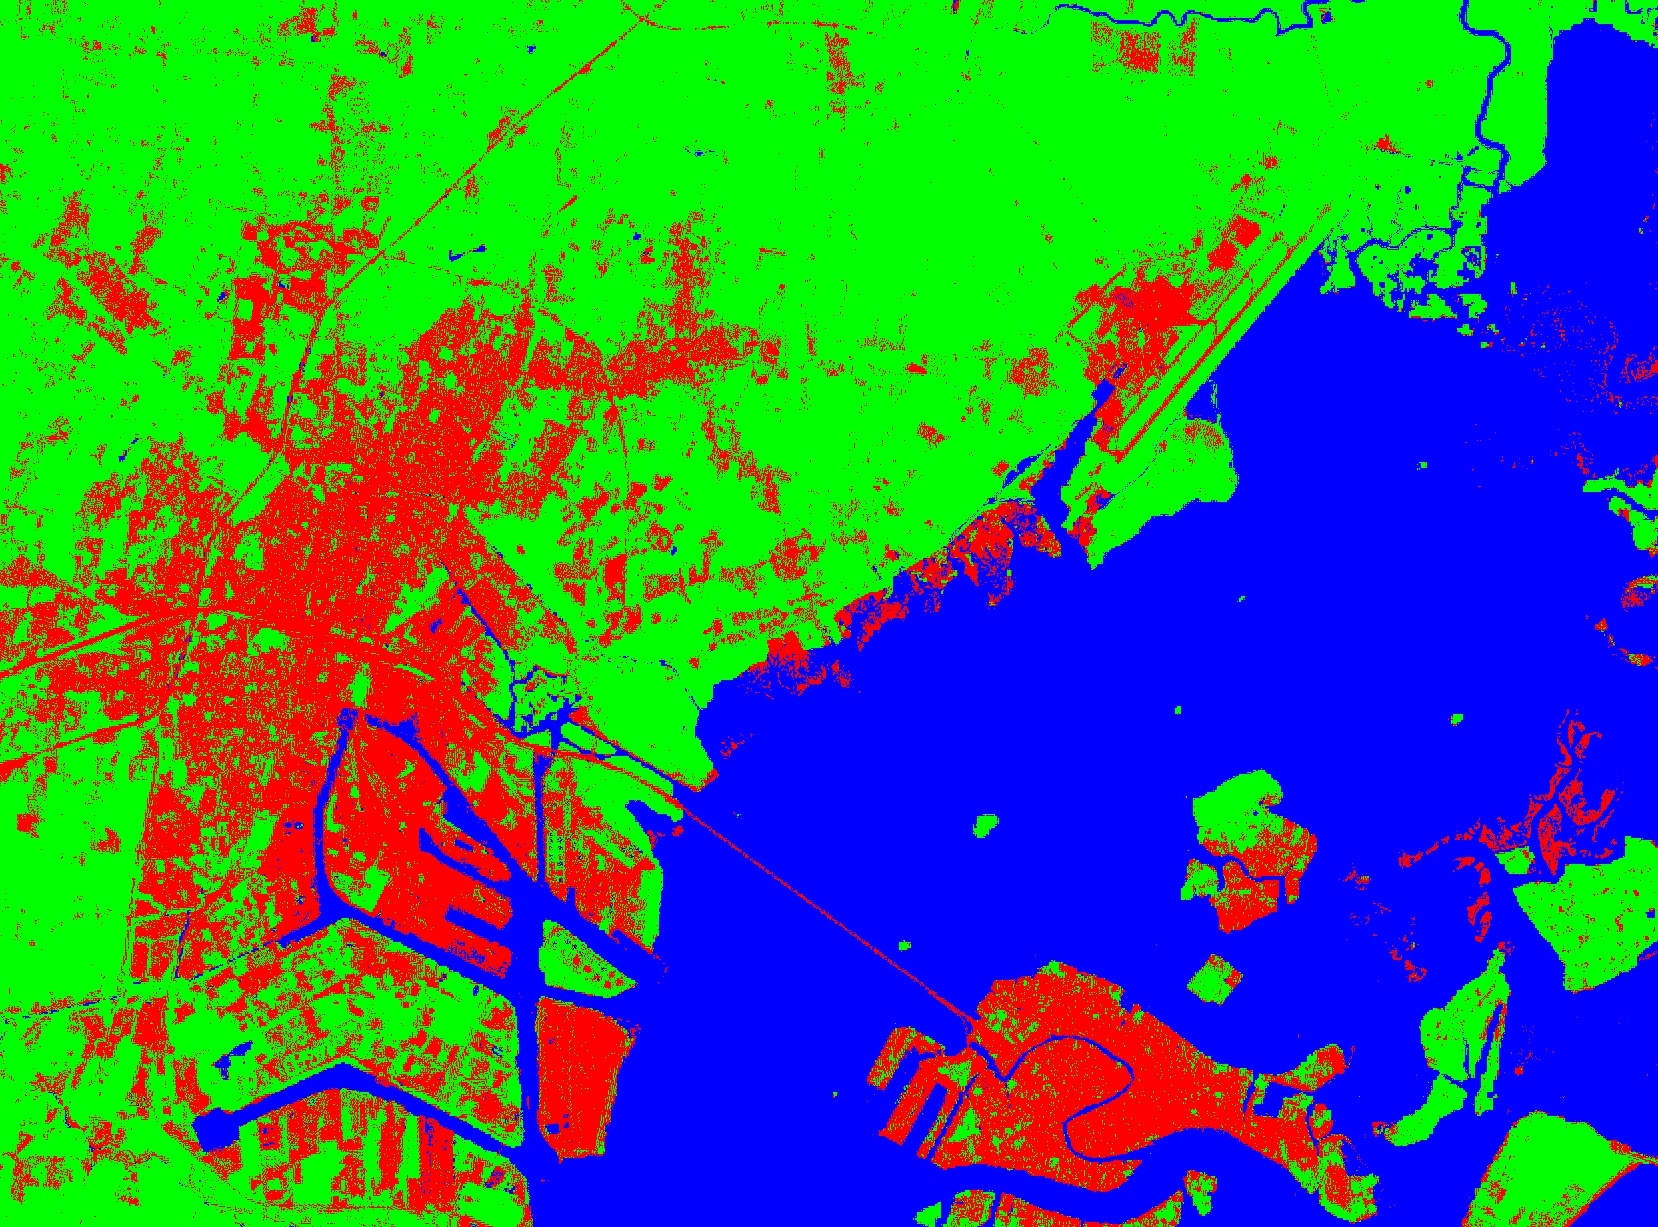
\includegraphics[height=250px]{LSE.png}
  \end{center}
\end{figure*}

\begin{figure*}
\begin{center}
  \caption{Superposition de l'image originale (en niveaux de gris) et de la classification des moindres carrés.}
  \label{veniseLSE}
  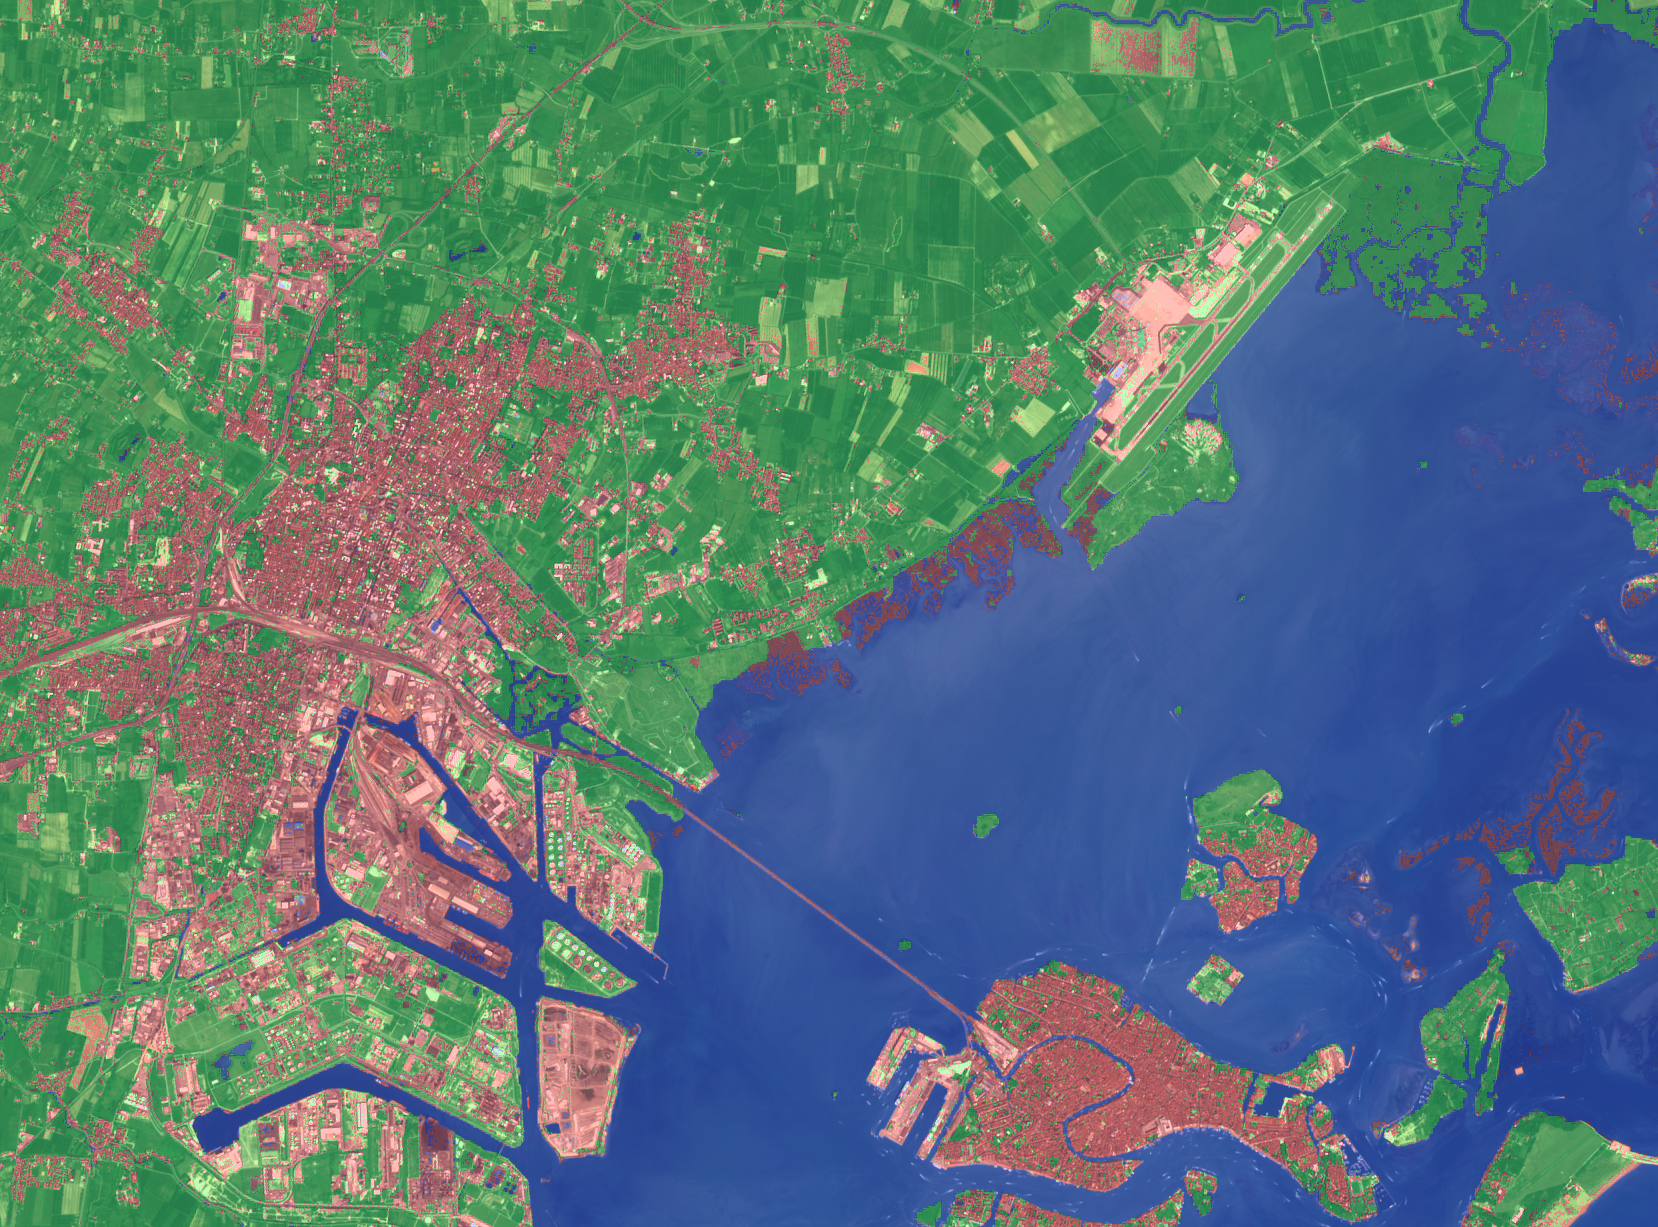
\includegraphics[height=250px]{veniseLSE.png}
  \end{center}
\end{figure*}

\begin{figure*}
\begin{center}
  \caption{Superposition de l'image originale (en niveaux de gris) et de la classification LDA.}
  \label{veniseLDA}
  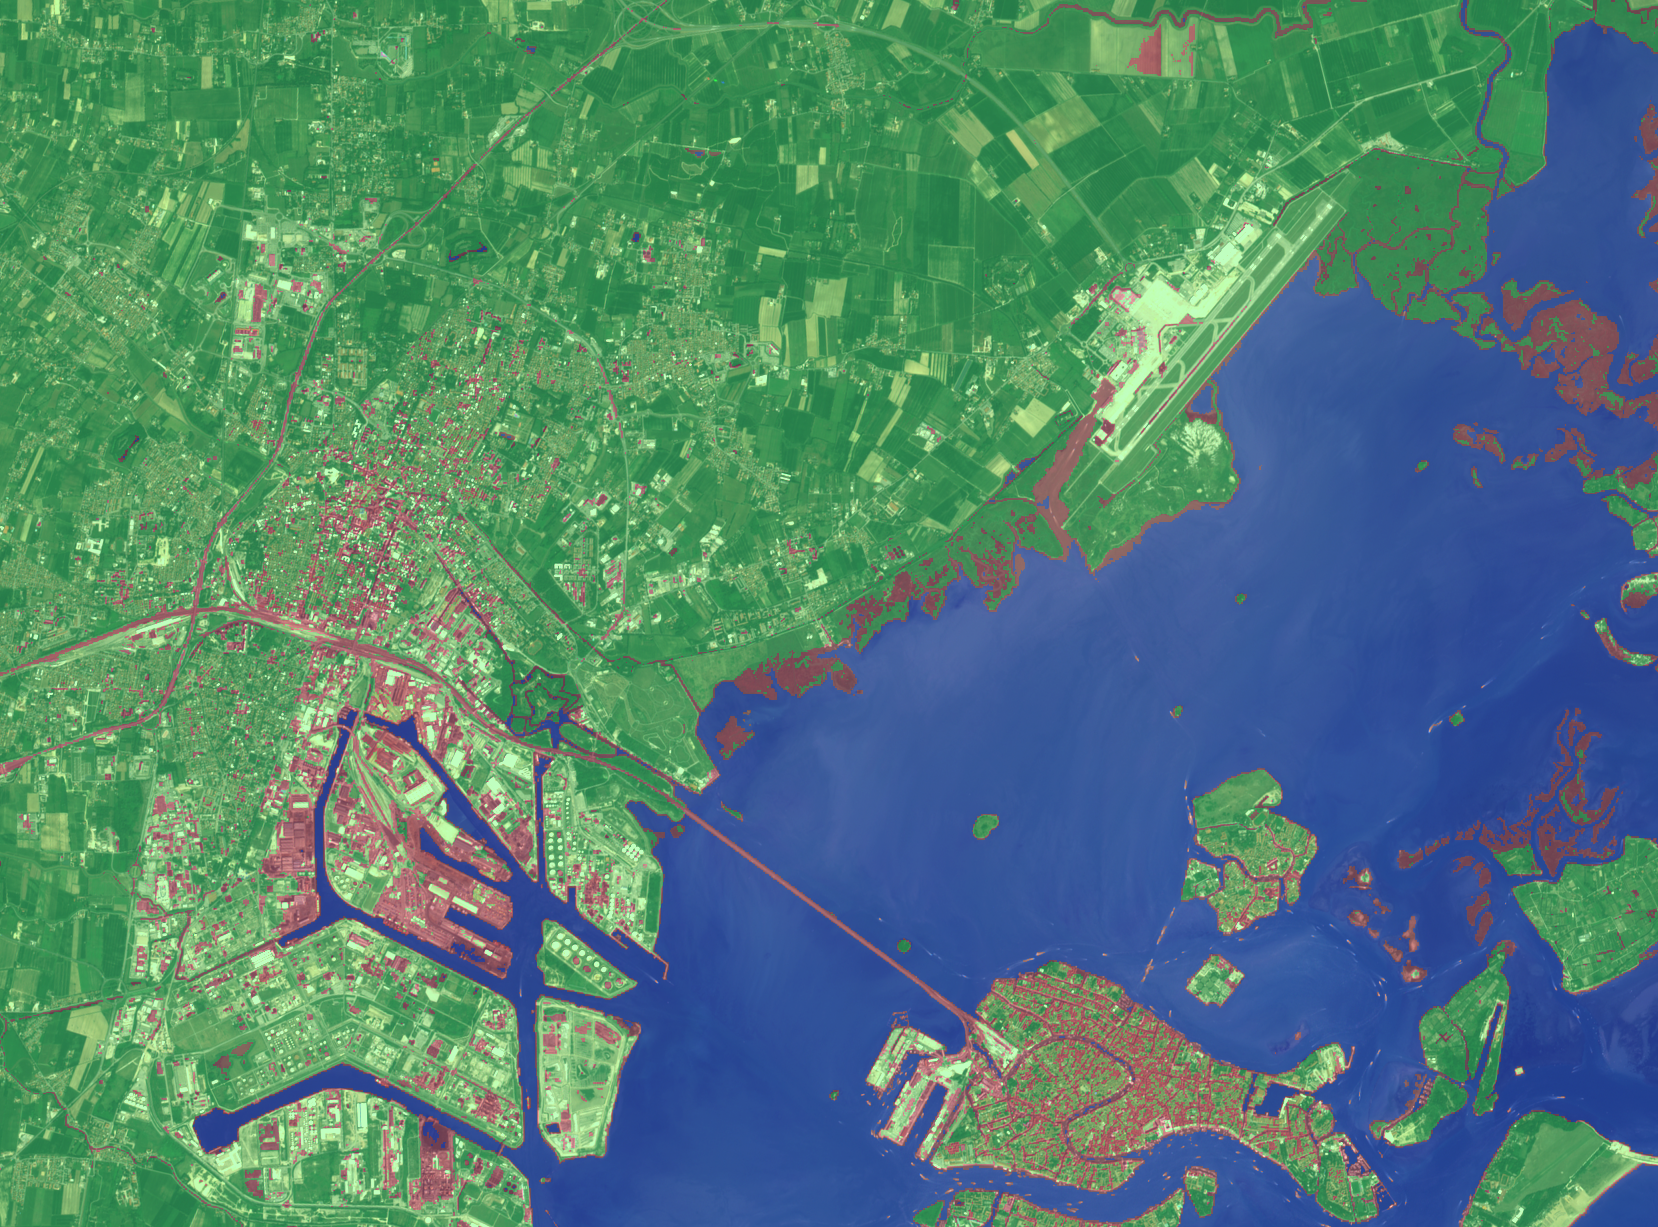
\includegraphics[height=250px]{veniseLDA.png}
  \end{center}
\end{figure*}

\begin{figure*}
\begin{center}
  \caption{Superposition de l'image originale (en niveaux de gris) et de la classification SVM.}
  \label{veniseSVM}
  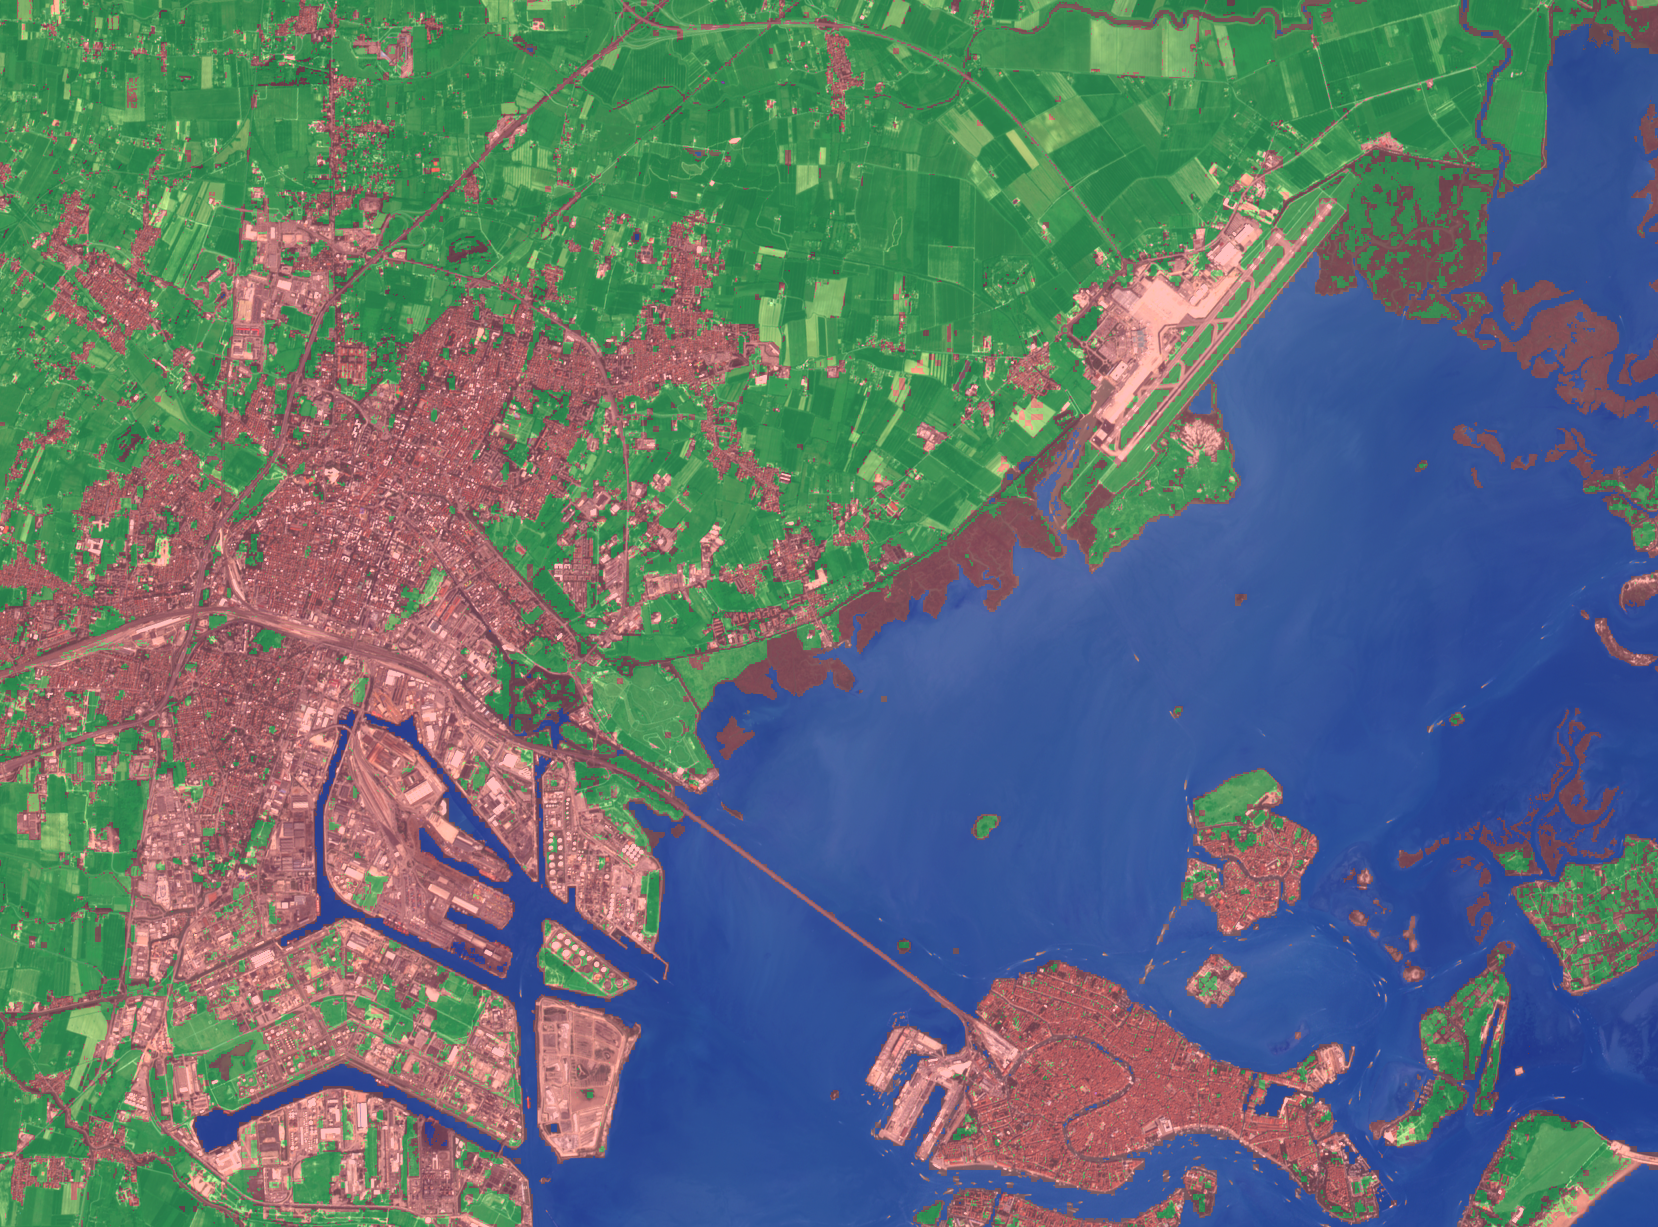
\includegraphics[height=250px]{veniseSVM.png}
  \end{center}
\end{figure*}

Cette classification n'est pas extrêmement précise, mais elle permet déjà de voir que la précision atteignable avec les images sentinel-2 semble supérieur à ce qui s'est fait par le passé.
\paragraph{L'analyse discriminante linéaire}
Cette méthode est encore plus simple à mettre en \oe{}uvre que la précédente, en effet, il suffit de calculer la moyenne et la variance des polygones d'entraînement. Cependant, cette classification est aussi beaucoup moins précise que celle des moindres carrés, et la précision diminue beaucoup plus vite avec la taille des polygones.\ref{veniseLDA}
\paragraph{Les machines à vecteurs de support}
Les SVM sont plus compliquées à implémenter, c'est pour cela que nous avons recours à la bibliothèque DLIB, qui nous permet d'avoir accès à des classes déjà définit que nous devons simplement réadapter à notre problème. Mais il faut aussi mettre en place un processus de validation croisée pour choisir les méta-paramètres de cette classification.\ref{veniseSVM}
\end{multicols}
\bibliography{Biblio}
\bibliographystyle{plain}
\end{document}
